\documentclass[12pt,a4paper]{article}
\usepackage{times}
\usepackage[utf8]{inputenc}
%\usepackage[english]{babel}
\usepackage[portuguese]{babel}
\usepackage[T1]{fontenc}
\usepackage{cite}
\usepackage{amsmath,amsfonts,amssymb} % pacote matematico
\usepackage{array}
\usepackage{graphicx,wrapfig}
\usepackage{float}
\usepackage{indentfirst}
\usepackage[inline]{enumitem}

\usepackage{psfrag}
\usepackage{pstricks}
\usepackage{epsfig}
\usepackage{url}           % Legenda no texto e na Lista de figuras diferentes. Habilita \cite{} na legenda.

\setlength{\parindent}{1.2cm}
\setlength{\parskip}{.2cm}
\setlength{\oddsidemargin}{0.5cm}    % Há um offset obrigatorio de
\setlength{\evensidemargin}{0.0cm}   % 1 inch do lado esquerdo e no
\setlength{\topmargin}{-1.2cm}       % topo da folha
\setlength{\headsep}{1.0cm}
\setlength{\textwidth}{15.5cm}
\setlength{\textheight}{24.2cm}
\renewcommand{\baselinestretch}{1.2}
\renewcommand{\labelitemi}{\tiny{\textbullet}}  % Define o ícone principal do itemize

%\hyphenation{Trans-ac-tions}

%\renewcommand{\contentsname}{Sumário}
\addto\captionsportuguese{
  \renewcommand{\contentsname}%
    {\hspace*{\fill}\bfseries\Large Sumário\hspace*{\fill}}%
}


\begin{document}
\pagenumbering{roman}

\begin{titlepage}
\thispagestyle{empty}
\begin{center}
\large{\bf{UFBA - Universidade Federal da Bahia}} \\
\large{\bf{Graduação em Engenharia da Computação}} \\
\end{center}
\vfill

\centering
\textbf{{\LARGE PLANO DE TRABALHO}}  \\ \vspace{0.5cm}
{\LARGE Graduação}
\vfill




\textbf{{\Large Sistema de Controle Remoto de Câmera Através de Sensores de um Smartfone}} \\ %\vspace{0.3cm}
%\hrulefill \\
\vfill
\begin{flushleft}
\textbf{Aluno}: Raffaello Salvetti Santos \hfill{}\\
\textbf{Orientador}: Paulo César Machado de Abreu Farias\hfill{}\\
\textbf{Linha de Pesquisa}: Robótica {\it ou} Sistemas Robóticos \hfill{}\\
\end{flushleft}

\vfill


\vspace{\stretch{1}}
\begin{center}
\large{\bf{\today}}
%\large{\bf{1 de Maio de 2019}}
\end{center}
\end{titlepage}


%---------------------------------------------------------------------------

\pagebreak
\begin{center}
\Large{\bf{Tabela de Modificações}}
\end{center}

\begin{center}
    \begin{tabular}{ | l | l | p{10cm} |}
    \hline
    Versão & Data & Resumo \\ \hline
    1.0 & 20/03/2018 & Inicial.\par Desenvolvimento de uma plataforma robótica com movimento diferencial, sensores e câmeras embarcadas. O robô pode ser controlado remotamente através de um joystic e sua câmera de navegação através da captura de movimento da cabeça do operador com sensores de um smartfone. As imagens da câmera de navegação são enviadas para o celular acoplado a cabeça do usuário.\\ \hline
    2.0 & 20/04/2019 & O escopo do projeto era extenso e foi reduzido.\par O projeto passa a ser a implementação de um sistema de controle para câmera (tilt, pan) operado remotamente orientado por sensores de posição disponíveis num smartfone acoplado a cabeça do usuário. \\ \hline
    \end{tabular}
\end{center}

\pagebreak


%---------------------------------------------------------------------------

\tableofcontents
\newpage

\pagenumbering{arabic}

\begin{abstract}
	Inspeção de áreas de difícil acesso ou que apresentam perigo, como dutos de ventilação, subestações de energia elétrica e reservatórios de produtos corrosivos, é uma realidade na indústria. O uso de robôs operados remotamente é uma solução que oferece segurança ao operador. O objetivo deste trabalho é desenvolver um sistema de controle remoto de câmera (embarcada num robô) usando os sensores de posição, disponíveis em smartfones, visando eficiência, versatilidade e baixo custo de produção.
\end{abstract}


%---------------------------------------------------------------------------------------------------------
\section{Introdução}
	Dutos de ventilação usados nos sistemas de ar-condicionado estão sujeitos a diversos tipos de danos, dentre os quais pode-se listar os entupimentos progressivos devido ao acúmulo de poeira e acúmulo de pequenos animais mortos. Por normalmente ser locais de difícil acesso, apresentam dificuldades em sua manutenção, favorecendo a proliferação de bactérias e transmissão de vírus\cite{carmo1999qualidade}\cite{bortoletto2002contaminaccao}.\par
	Subestações de energia elétrica, em grande parte das vezes, ficam expostas a intempéries, que causam oxidações em suportes, equipamentos e cabos. Sua inspeção oferece riscos a vida por expor o corpo humano a uma quantidade enorme de energia, apesar de existir norma rigorosa para a realização de inspeções preventivas, acidentes com vítima ainda acontecem\cite{santos2012inspeccao}.\par
	A inspeção de reservatórios de produtos químicos requer uma minuciosa análise estrutural, uma busca por áreas oxidadas e falhas em pontos de solda, que demanda muitas horas de trabalho humano. A exposição a gases e vapores tóxicos, por menor que seja a quantidade, causam riscos a saúde do inspetor\cite{souza2012inspeccao}\cite{molina2008metodo}.\par
	Os exemplos acima, são apenas algumas das atividades extremamente necessárias no ambiente industrial, que expõem pessoas a riscos de morte e que podem ser evitados através de dispositivos especializados. Os dispositivos usados para esse fim, são robôs equipados com ferramentas adequadas para cada tarefa, que podem oferecer um sistema de navegação autônomo ou de controle remoto.

%---------------------------------------------------------------------------------------------------------
\section{Objetivo}
	O objetivo deste trabalho é a construção de um sistema de controle remoto para câmeras de navegação, usando sensores de posição disponíveis em smartfones, que podem ser usadas em robôs de inspeção.\par
	O dispositivo oferecerá uma visão imersiva ao operador, trazendo a sensação de estar presente no local de inspeção.\par
	Usando atuadores, a câmera poderá ser movimentada com base nos movimentos da cabeça do operador. Esses movimentos são capturados por um smartfone acoplado à cabeça do usuário através de um óculos especial, tornando intuitivo o controle de câmera e diminuindo a quantidade de ações manuais necessárias para operar o dispositivo.

%---------------------------------------------------------------------------------------------------------
\section{Metodologia}
	É necessário construir um suporte para dois servo motores, um para a função \emph{tilt}\footnote{Inclinar em inglês.} (movimento vertical em relação a imagem da câmera) e um para a função \emph{pan}\footnote{Derivado de "panning", que significa girar horizontalmente a partir de um ponto fixo em inglês.} (movimento horizontal em relação a imagem da câmera). Além de posicionar os motores de forma perpendicular aos respectivos eixos, o suporte tem a função de fixar a câmera.\par
	O controle de movimento dos motores será feito com um \emph{Raspberry Pi 1 modelo B}\footnote{Um micro computador do tipo SOC, do inglês "System on a Chip", ou computador num único chip.} que aciona os motores através de PWM\footnote{Modulação por largura de pulso.}.\par
	Os softwares de operação serão desenvolvidos como módulos da solução nas linguagens Java (Android), python e C/C++ (Raspberry Pi).\par
	Os módulos serão: \begin{enumerate*} \item um aplicativo que deverá rodar num celular Android, responsável por capturar dados relativos a posição e movimentação da cabeça do operador e enviar para o Raspberry Pi; \item um programa rodará num Raspberry PI e será responsável por traduzir os dados referentes aos movimentos da cabeça do operador em movimentos dos servo motores.\end{enumerate*}\par

\subsection{Diagrama de Blocos}
\begin{figure}[H]
	\centering
	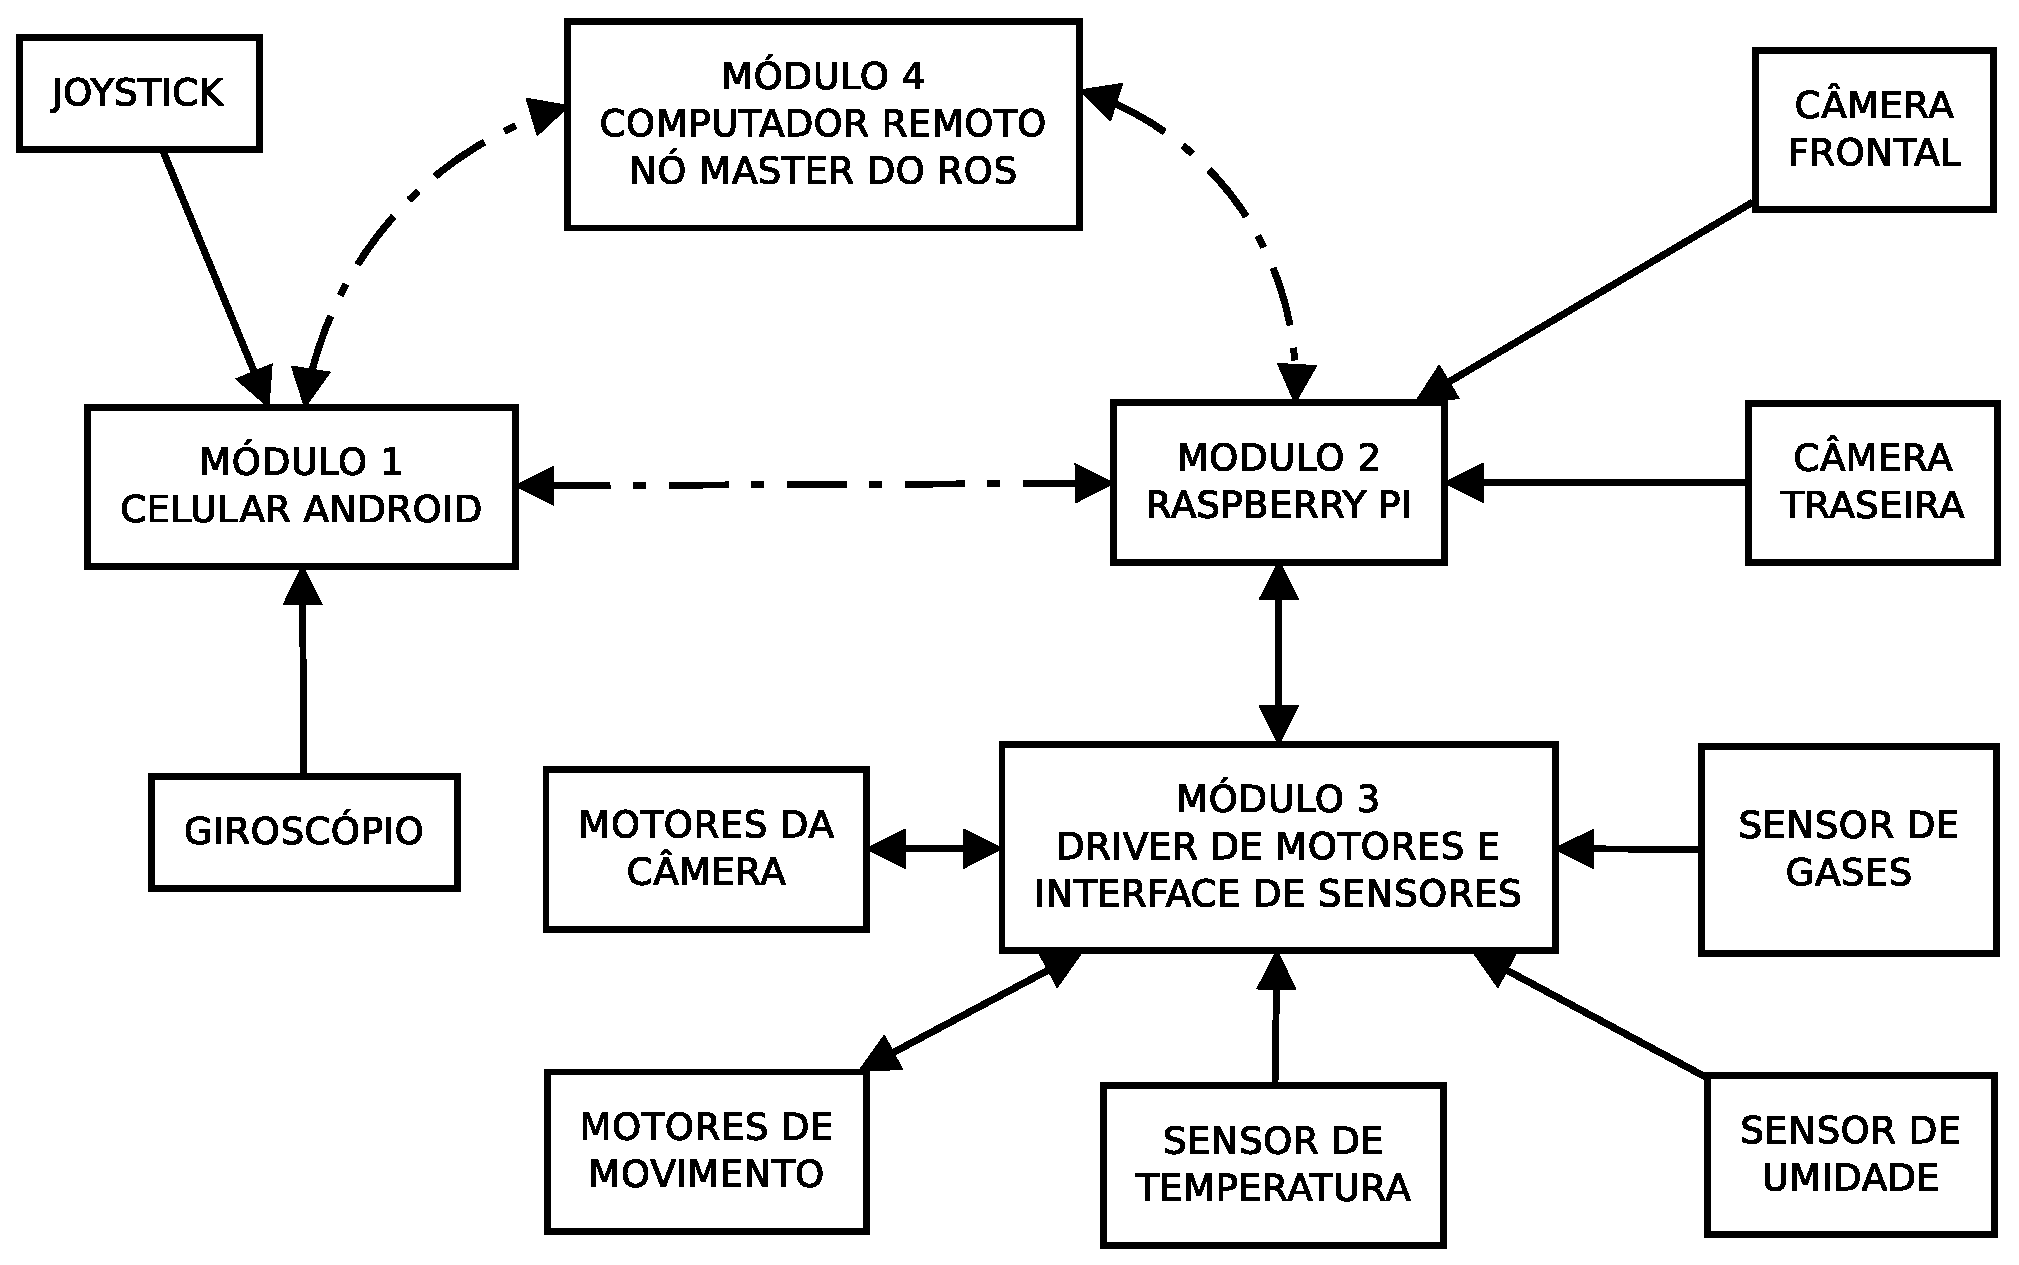
\includegraphics[scale=0.45]{diagrama-modulos} 
	\label{fig:diag-modulos}
	\caption{Diagrama de blocos da solução.}
\end{figure}

\subsection{Descrição dos Módulos \label{sec:desc-modulos}}
\begin{enumerate}
\item \textbf{Módulo do Celular Android - Visualização Imersiva\label{mod:celular}}\\
	Esse módulo captura dados referentes a posição da cabeça do operador (usando os sensores giroscópio, acelerômetro e magnetômetro), aplica os filtros necessários nos dados e os envia para o módulo \ref{mod:raspi}. Esse módulo também é responsável por receber as imagens da câmera capturadas pelo módulo \ref{mod:raspi}. Será usado um celular juntamente com um \emph{óculos VR Cardboard}\footnote{Óculos de realidade virtual criado pelo Goole como kit de desenvolvimento básico para aplicações imersivas.} como um display para mostrar o vídeo e transmitido pela câmera, dando a ideia de imersão.
\item \textbf{Módulo de Controle Embarcado - Raspberry PI\label{mod:raspi}}\\
	Esse módulo será um programa escrito em python e rodará num Raspberry PI 1 modelo B, que possui um processador \emph{ARM}\footnote{Do inglês, Advanced RISC Machine. É uma arquitetura de processadores com um numero reduzido de instruções e de baixo custo de produção.} de 700MHz, 512Mb de memória RAM, 26 \emph{GPIO}\footnote{Pinos de propósito geral.}, duas portas USB e uma porta Ethernet. Será responsável por receber os dados dos sensores de posição enviado pelo módulo \ref{mod:celular} e converterá tais dados em PWM (através dos pinos GPIO) para ambos servo motores (tilt e pan), além de enviar as imagens da câmera para o módulo \ref{mod:celular}, lidar com as conexões de rede ethernet via cabo ou rede sem fio.
\end{enumerate}

\subsection{Conhecimento Necessário}
	Para construir os módulos listados na seção \ref{sec:desc-modulos}, se faz necessário os seguintes conhecimentos:
\begin{enumerate}[noitemsep]
	\item Eletrônica Geral
	\item Fontes de Alimentação
	\item Supressão de Ruído (Interferência Eletromagnética dos servo motores)
	\item Acionamento de Motores atraves de PWM
	\item Sistema Operacional Linux
	\item Sistema Operacional Android
	\item Linguagens de Programação (Java, Python e C/C++)
	\item Android SDK (Cardboard SDK)
	\item Redes de Computadores (Ethernet)
\end{enumerate}

%---------------------------------------------------------------------------------------------------------
\section{Resultados Esperados}
	Espera-se que, com os conhecimentos obtidos no curso de Engenharia da Computação, seja possível construir um sistema de controle de camera com as características descritas. Após a construção, o sistema será testado em ambiante controlado para que se observe parâmetros estabilidade e confiabilidade.


%---------------------------------------------------------------------------------------------------------
%\section*{Referências Bibliográficas}
% OBSERVAÇÃO: A seção de referências deve ser gerada automaticamente usando os comandos \cite{} do LaTex. Estou usando o padrão IEEE para citações.

\nocite{*}
\bibliography{bibliografia}
\bibliographystyle{ieeetr}

\end{document}
